\documentclass[11pt,a4paper]{article}
\usepackage[T1]{fontenc}
\usepackage[utf8]{inputenc}
\usepackage[a4paper,left=22mm,right=22mm,top=21mm,bottom=23mm,headsep=7mm]{geometry}
\usepackage{amsmath,amssymb,mathtools,amsthm}
\usepackage{newtxtext,newtxmath}
\usepackage{microtype,booktabs,array}
\usepackage{xcolor,tikz}
\usetikzlibrary{arrows.meta,calc,positioning,fit,backgrounds,decorations.pathreplacing}
\usepackage[font=small,labelfont=bf,labelsep=period]{caption}
\usepackage{titlesec,fancyhdr}
\usepackage[colorlinks=true,linkcolor=ink,citecolor=ink,urlcolor=ink]{hyperref}
\definecolor{ink}{HTML}{233C53}
\definecolor{pathblue}{HTML}{237A9C}
\definecolor{target}{HTML}{B76533}
\definecolor{tailgreen}{HTML}{307E6B}
\definecolor{violet}{HTML}{75618D}
\definecolor{pale}{HTML}{EDF3F6}
\definecolor{grey}{HTML}{87929B}
\hypersetup{pdftitle={From edge to bulk in free fermions in disguise},pdfsubject={An explicit partial inverse problem at infinite temperature},pdfauthor={Istvan Vona}}
\author{Istvan Vona}
\date{10 November 2026}
\pagestyle{fancy}\fancyhf{}
\fancyhead[L]{\footnotesize\scshape From edge to bulk in free fermions in disguise}
\fancyhead[R]{\footnotesize Expository letter}
\fancyfoot[C]{\small\thepage}
\renewcommand{\headrulewidth}{0.3pt}
\setlength{\headheight}{14pt}
\titleformat{\section}{\large\bfseries\color{ink}}{\thesection.}{.6em}{}
\titleformat{\subsection}{\normalsize\bfseries}{\thesubsection.}{.5em}{}
\titlespacing*{\section}{0pt}{2.2ex plus .4ex minus .2ex}{.8ex}
\titlespacing*{\subsection}{0pt}{1.5ex plus .3ex}{.6ex}
\setlength{\parindent}{1em}
\setlength{\parskip}{.15em}
\setlength{\textfloatsep}{12pt plus 2pt minus 2pt}
\setlength{\floatsep}{10pt plus 2pt minus 2pt}
\setlength{\intextsep}{10pt plus 2pt minus 2pt}
\setlength{\abovedisplayskip}{8pt plus 2pt minus 2pt}
\setlength{\belowdisplayskip}{8pt plus 2pt minus 2pt}
\allowdisplaybreaks[1]
\newcommand{\ii}{\mathrm i}
\newcommand{\tr}{\operatorname{Tr}}
\newcommand{\av}[1]{\langle #1\rangle_\infty}
\newcommand{\HH}{\mathcal H}
\newcommand{\LL}{\mathcal L}
\newcommand{\eps}{\varepsilon}
\newcommand{\Sig}{\mathcal I}
\newcommand{\Kern}{\mathcal K}
\newcommand{\W}{\mathcal W}
\newcommand{\one}{\mathbf 1}
\newcommand{\PP}[1]{P_{[#1]}}
\newtheorem{theorem}{Theorem}
\tikzset{site/.style={circle,draw=ink,fill=white,minimum size=5.5mm,inner sep=0pt,font=\small},
 psite/.style={site,draw=pathblue,fill=pathblue!12,line width=.8pt},
 tsite/.style={site,draw=target,fill=target!16,line width=.9pt},
 source/.style={circle,draw=violet,fill=violet!12,minimum size=7mm,inner sep=0pt,font=\small},
 bg/.style={draw=grey!55,line width=.5pt},
 pe/.style={draw=pathblue,line width=1.25pt},
 te/.style={draw=target,line width=1.25pt},
 se/.style={draw=violet,line width=.9pt},
 lab/.style={font=\small,align=left}}
\begin{document}
\thispagestyle{plain}
\begin{center}
{\small\scshape\color{ink} Exact dynamics\enspace /\enspace Partial inverse problem}\par\vspace{8pt}
{\LARGE\bfseries From edge to bulk in\par free fermions in disguise}\par\vspace{5pt}
{\large Explicit density correlators from induced paths}\par\vspace{7pt}
{\normalsize Istvan Vona}\par\vspace{4pt}
{\small 10 November 2026}
\end{center}
\vspace{-2pt}
\begin{abstract}
A free-fermion spectrum does not by itself determine local spin correlation functions. For the open free-fermions-in-disguise chain, however, each of the first three Hamiltonian terms, and by reflection each of the last three, has an explicitly computable infinite-temperature dynamical correlator with every term in the chain. We derive these correlators in three steps: the end-to-end density correlator, boundary sources coupled to a clique of up to three terms, and a target moved into the bulk. The mechanism is trace orthogonality: two induced-path products survive precisely when their vertex sets differ by the target vertex. At the endpoint this gives one scalar path polynomial; in the bulk only two terminal configurations and three residual interval polynomials are needed. Using unnormalized spectral residues removes all fermion-normalization factors, while a uniform subtraction accounts for stationary source components without casework. The resulting finite double sums require polynomial arithmetic work in system size. The derivation does not reconstruct a generic bulk operator or solve the bulk--bulk inverse problem.
\end{abstract}

\section{The question and the chain}
Fendley's open chain has a free-fermion spectrum even though its local terms are not ordinary Jordan--Wigner fermion bilinears~\cite{Fendley,Elman,Chapman}. The inverse problem asks for the converse dictionary: which local spin operators can be expressed simply using the hidden modes? Boundary-operator dynamics was obtained by Vona, Mesty\'an and Pozsgay~\cite{VMP}. The path-product expansion of Fukai, Pozsgay and Vona~\cite{FPV} now makes the operator content of the modes explicit. Here we use that expansion to evaluate density correlators without solving the full inverse problem for the bulk density.

Let
\begin{equation}
\HH=\sum_{j=1}^{M}h_j,\qquad h_j=b_jg_j,\qquad B_j=b_j^2>0,
\qquad
 g_j^2=1,\quad
 g_ig_j=(-1)^{\mathbf1_{0<|i-j|\le2}}g_jg_i.
\label{eq:model}
\end{equation}
The couplings $b_j$ may have either sign. The frustration graph has one vertex for each $h_j$ and an edge for every anticommuting pair: it is the square of an open path, not the ordinary path. We fix the spin realization
\begin{equation}
 g_j=Z_{j-2}Z_{j-1}X_j,\qquad Z_0=Z_{-1}=1,
 \qquad
 \av{A}=2^{-M}\tr A,\qquad A(t)=e^{\ii\HH t}Ae^{-\ii\HH t}.
 \label{eq:rep}
\end{equation}
The ordered words $g_A=\prod_{j\in A}^{\uparrow}g_j$ are trace-orthonormal:
$\av{g_A^\dagger g_C}=\delta_{A,C}$. Thus a nonempty word has zero trace. This is the trace convention used throughout; no projection onto a particular symmetry sector is made. Our observables are the \emph{coupled terms} $h_j$. Divide $\av{h_i(t)h_j}$ by $b_ib_j$ to obtain the correlator of $g_i,g_j$.

\begin{figure}[t]
\centering
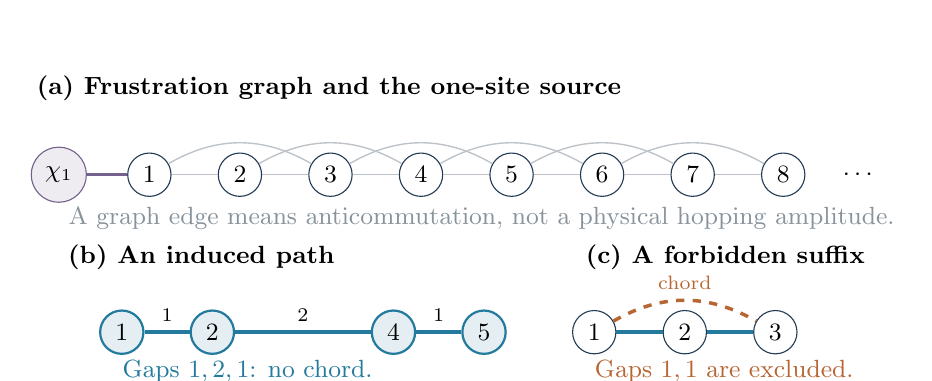
\begin{tikzpicture}[x=1.15cm,y=1cm]
\node[lab,font=\small\bfseries,anchor=west] at (-.35,1.1) {(a) Frustration graph and the one-site source};
\foreach \i in {1,...,8}{\node[site] (g\i) at (\i,0) {$\i$};}
\node[source] (ch) at (0,0) {$\chi_1$};
\foreach \i in {1,...,7}{\pgfmathtruncatemacro{\j}{\i+1}\draw[bg] (g\i)--(g\j);}
\foreach \i in {1,...,6}{\pgfmathtruncatemacro{\j}{\i+2}\draw[bg] (g\i) to[bend left=30] (g\j);}
\draw[se] (ch)--(g1);
\node[lab,anchor=west] at (8.55,0) {$\cdots$};
\node[lab,anchor=west,text=grey] at (0,-.55) {A graph edge means anticommutation, not a physical hopping amplitude.};
\begin{scope}[yshift=-2cm,xshift=8mm]
\node[lab,font=\small\bfseries,anchor=west] at (-.7,.95) {(b) An induced path};
\foreach \x/\a in {0/1,1/2,3/4,4/5}{\node[psite] (p\a) at (\x,0) {$\a$};}
\draw[pe] (p1)--node[above,font=\scriptsize] {$1$}(p2);
\draw[pe] (p2)--node[above,font=\scriptsize] {$2$}(p4);
\draw[pe] (p4)--node[above,font=\scriptsize] {$1$}(p5);
\node[lab,anchor=west,text=pathblue] at (-.1,-.5) {Gaps $1,2,1$: no chord.};
\end{scope}
\begin{scope}[yshift=-2cm,xshift=68mm]
\node[lab,font=\small\bfseries,anchor=west] at (-.2,.95) {(c) A forbidden suffix};
\foreach \x/\a in {0/1,1/2,2/3}{\node[site] (f\a) at (\x,0) {$\a$};}
\draw[pe] (f1)--(f2)--(f3);
\draw[te,dashed] (f1) to[bend left=30] node[above,font=\scriptsize,text=target] {chord} (f3);
\node[lab,anchor=west,text=target] at (-.1,-.5) {Gaps $1,1$ are excluded.};
\end{scope}
\end{tikzpicture}
\caption{The graph behind the calculation. An induced path contains no edge between nonconsecutive path vertices. From a left boundary source, its physical vertices increase monotonically, with gaps $1$ or $2$, and never two successive gaps $1$. These local rules will replace an exponentially large operator expansion by a scalar recurrence.}
\label{fig:graph}
\end{figure}

For an interval, define its weighted independence polynomial by
\begin{equation}
 \PP{a,b}(x)=\sum_{\substack{I\subseteq[a,b]\\ |i-j|>2\ (i\ne j)}}
 (-x)^{|I|}\prod_{i\in I}B_i,\qquad \PP{a,b}=1\quad(a>b).
 \label{eq:Pdef}
\end{equation}
Selecting or omitting the last vertex gives
\begin{equation}
 \PP{a,m}(x)=\PP{a,m-1}(x)-xB_m\PP{a,m-3}(x).
 \label{eq:Prec}
\end{equation}
Write $P(x)=\PP{1,M}(x)$ and $S=\lceil M/3\rceil$. We first assume simple roots $x_a=u_a^2>0$, and use signed labels
\begin{equation}
 \Sig=\{-S,\ldots,-1,1,\ldots,S\},\qquad
 u_{-a}=-u_a,\quad \eps_s=u_s^{-1},\quad P'_s=P'(u_s^2).
 \label{eq:roots}
\end{equation}
These are the single-particle energies: the spectrum is built from signed sums of the positive $\eps_a$~\cite{Fendley,Elman}. Singular parameter choices are obtained by continuity of the final finite-dimensional correlator, not by substituting into an individual singular residue.

\section{A boundary source turns dynamics into residues}
Start with $\chi_1=Z_1$. It anticommutes only with $h_1$, so
\begin{equation}
 \LL(A):=\tfrac12[\HH,A],\qquad
 \LL(\chi_1)=h_1\chi_1,\qquad h_1=\LL(\chi_1)\chi_1.
 \label{eq:source}
\end{equation}
Thus it suffices to evolve the source and its commutator. Add a source vertex $\alpha_1$ adjacent only to vertex $1$. A rooted induced path $p$ has physical vertices $(i_1,\ldots,i_n)$, and path word
\begin{equation}
 \Pi_p=\chi_1h_{i_1}\cdots h_{i_n},\qquad \Pi_{\varnothing}=\chi_1.
\end{equation}
Remove the path and every vertex adjacent to it, including those adjacent to the source. The remaining physical graph is the \emph{residual graph} $\overline p$. For the empty path it is $[2,M]$; for a nonempty path ending at $r$ it is $[r+3,M]$. The latter fact follows directly from the gap rule in Fig.~\ref{fig:graph}.

The path-product numerator and its resolvent are
\begin{equation}
 \Xi_1(u)=\sum_p(-u)^{|p|}P_{\overline p}(u^2)\Pi_p,
 \qquad
 \Phi_1(u)=\frac{\Xi_1(u)}{P(u^2)}=(1-u\LL)^{-1}\chi_1.
 \label{eq:Xi}
\end{equation}
Here $|p|$ counts physical vertices. The equality is the path-product identity of Ref.~\cite{FPV}, specialized to this chain. Its useful local form is
\begin{equation}
 u\LL\Xi_1(u)=\Xi_1(u)-P(u^2)\chi_1.
 \label{eq:resolventidentity}
\end{equation}
It can be understood without diagonalizing a spin Hamiltonian. In a commutator, an internal path vertex has two path neighbors and hence contributes nothing. The endpoint can be removed or extended; the residual-polynomial recurrence accounts for these two operations. Terms that insert a chord cancel between the corresponding alternative parent paths. The surviving empty-path term is exactly $-P(u^2)\chi_1$. Ref.~\cite{FPV} proves this cancellation and the associated fermionic algebra; the correlator derivations below require only \eqref{eq:resolventidentity} and the explicit path words.

\paragraph{A normalization-free choice.}
Instead of introducing normalized fermions and their source coefficients separately, take the spectral components of $\chi_1$ directly:
\begin{equation}
 F_s^{(1)}=-\frac{\Xi_1(u_s)}{2u_s^2P'_s},\qquad
 \LL F_s^{(1)}=\eps_sF_s^{(1)}.
 \label{eq:F}
\end{equation}
The sign and factor follow from the residue at $u=u_s$:
$\operatorname{Res}\Phi_1=\Xi_1(u_s)/(2u_sP'_s)$, whereas
$\operatorname{Res}(1-u/u_s)^{-1}F_s^{(1)}=-u_sF_s^{(1)}$.
Partial fractions therefore give
\begin{equation}
 \chi_1(t)=Z_1^{\rm st}+\sum_{s\in\Sig}e^{2\ii t\eps_s}F_s^{(1)},
 \qquad [\HH,Z_1^{\rm st}]=0,\qquad
 Z_1^{\rm st}=\chi_1-\sum_sF_s^{(1)}.
 \label{eq:sourceevol}
\end{equation}
The superscript distinguishes the stationary operator $Z_1^{\rm st}$ from the Pauli matrix $Z_1$. No explicit construction of this stationary part will be needed.

For comparison with normalized modes, set $Q_1(x)=\PP{2,M}(x)$,
$N_s^{(1)}=2\sqrt{-u_s^2Q_1(u_s^2)P'_s}$ and
$\Psi_s^{(1)}=\Xi_1(u_s)/N_s^{(1)}$. Then
$F_s^{(1)}=d_s^{(1)}\Psi_s^{(1)}$ with
$d_s^{(1)}=2Q_1(u_s^2)/N_s^{(1)}$ and
$\{\Psi_s^{(1)},\Psi_r^{(1)}\}=\delta_{s+r,0}$~\cite{FPV}.
Equation~\eqref{eq:F} is simply this product with its normalization factors cancelled.

\section{First calculation: the end-to-end correlator}
\subsection{One path polynomial}
Let $R_m(y)$ sum all induced paths from $1$ to $m$, weighting every physical vertex \emph{except the final one} by $-yB_i$:
\begin{equation}
 R_m(y)=\sum_{p:1\leadsto m}\prod_{i\in V(p)\setminus\{m\}}(-yB_i).
 \label{eq:R}
\end{equation}
There are only two terminal possibilities: a final jump $m-2\to m$, or a final pair of jumps $m-3\to m-1\to m$. Consequently
\begin{align}
 R_1=1,\qquad R_2=R_3=-yB_1,\qquad
 R_m&=-yB_{m-2}R_{m-2}+y^2B_{m-3}B_{m-1}R_{m-3}
 \quad(m\ge4).
 \label{eq:Rrec}
\end{align}
For example $R_4=y^2B_1(B_2+B_3)$ and
$R_5=y^2B_1B_3-y^3B_1B_2B_4$. The terminal coupling $B_m$ is absent: the observable insertion will supply it.

\subsection{Trace orthogonality pairs a path with its extension}
Consider the unnormalized overlap
\begin{equation}
 \Kern_{1M}(u,v):=\av{\Xi_1(u)\Xi_1(v)h_M}.
\end{equation}
In a product of two path words the two source factors disappear. The trace can then be nonzero only if
\begin{equation}
 V(p)\mathbin{\triangle}V(q)=\{M\},
 \label{eq:selection}
\end{equation}
where $\triangle$ is symmetric difference. Hence the paths are a common prefix $\rho$ and its one-vertex extension $\rho M$. Both residual graphs are empty: the prefix already ends at $M-1$ or $M-2$. This is why no right-tail polynomial remains.

\begin{figure}[t]
\centering
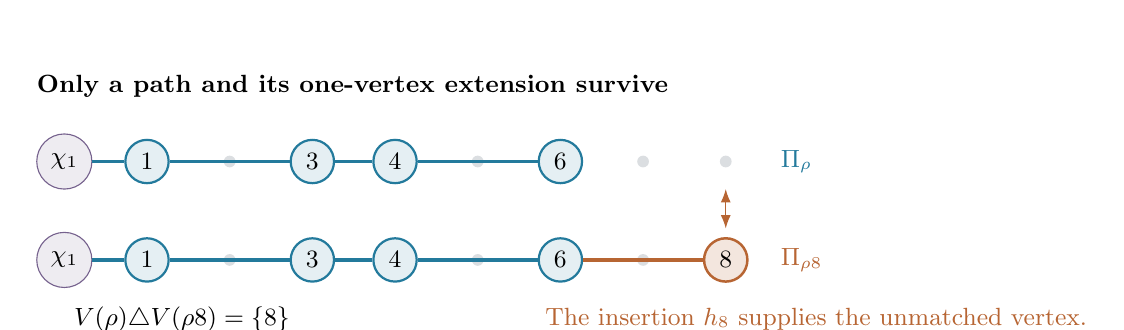
\begin{tikzpicture}[x=1.05cm,y=1cm]
\node[lab,font=\small\bfseries,anchor=west] at (-.45,1.95) {Only a path and its one-vertex extension survive};
\foreach \yy/\tag in {1/a,-.25/b}{
 \node[source] (s\tag) at (0,\yy) {$\chi_1$};
 \foreach \i in {1,...,8}{\node[circle,fill=grey!30,inner sep=1.5pt] (\tag\i) at (\i,\yy) {};}
 \foreach \i in {1,3,4,6}{\node[psite] (\tag\i) at (\i,\yy) {$\i$};}
 \draw[pe] (s\tag)--(\tag1)--(\tag3)--(\tag4)--(\tag6);
}
\node[tsite] (b8) at (8,-.25) {$8$};
\draw[te] (b6)--(b8);
\node[lab,text=pathblue,anchor=west] at (8.55,1) {$\Pi_\rho$};
\node[lab,text=target,anchor=west] at (8.55,-.25) {$\Pi_{\rho 8}$};
\draw[<->,>=Latex,draw=target] (8,.15)--(8,.65);
\node[lab,text=target,anchor=west] at (5.7,-1) {The insertion $h_8$ supplies the unmatched vertex.};
\node[lab,anchor=west] at (0,-1) {$V(\rho)\triangle V(\rho8)=\{8\}$};
\end{tikzpicture}
\caption{The end-to-end trace selection, illustrated at $M=8$. The two paths have the same prefix $(1,3,4,6)$; one ends at $6$, and the other appends $8$. The closed neighborhood of either path reaches the end of the chain. Reversing their order changes the trace sign, producing the antisymmetric factor $u-v$.}
\label{fig:pair}
\end{figure}

To see the sign explicitly, let $n=|\rho|$ and $B_\rho=\prod_{i\in\rho}B_i$. The two traces are
\begin{equation}
 \av{\Pi_\rho\Pi_{\rho M}h_M}=(-1)^nB_MB_\rho,
 \qquad
 \av{\Pi_{\rho M}\Pi_\rho h_M}=(-1)^{n-1}B_MB_\rho.
\end{equation}
Multiplying by $(-u)^n(-v)^{n+1}$ and $(-u)^{n+1}(-v)^n$, respectively, gives
$B_M(u-v)(-uv)^nB_\rho$. Summing the prefixes proves
\begin{equation}
 \boxed{\Kern_{1M}(u,v)=B_M(u-v)R_M(uv).}
 \label{eq:endkernel}
\end{equation}
This identity holds for arbitrary $u,v$, not just at spectral roots.

\subsection{A uniform treatment of stationary components}
From \eqref{eq:source}, $h_1(t)=(\sum_s\eps_se^{2\ii t\eps_s}F_s^{(1)})\chi_1(t)$. The remaining stationary matrix element can be eliminated at time zero. For $M>1$,
\begin{equation}
 \av{F_s^{(1)}\chi_1h_M}=0,
 \qquad
 \av{F_s^{(1)}Z_1^{\rm st}h_M}
 =-\sum_r\av{F_s^{(1)}F_r^{(1)}h_M}.
 \label{eq:zeroelim}
\end{equation}
Indeed, a single source path cannot have physical vertex set $\{M\}$.
The first equality is a selection rule, not an assumption that the stationary part vanishes.
Define the common spectral weight
\begin{equation}
 \W_{sr}(t)=
 \frac{e^{2\ii t(\eps_s+\eps_r)}-e^{2\ii t\eps_s}}
 {4u_s^3u_r^2P'_sP'_r}.
 \label{eq:weight}
\end{equation}
Equations~\eqref{eq:F}, \eqref{eq:endkernel} and \eqref{eq:zeroelim} yield the first answer:
\begin{equation}
 \boxed{\av{h_1(t)h_M}
 =B_M\sum_{s,r\in\Sig}\W_{sr}(t)(u_s-u_r)R_M(u_su_r),\qquad M>1.}
 \label{eq:endcorr}
\end{equation}
When $Z_1^{\rm st}=0$, the subtraction in \eqref{eq:weight} sums to zero; when it is present, the same subtraction includes its effect exactly. No congruence-class switch is needed. Moreover $\W_{sr}(0)=0$, so the off-diagonal equal-time answer vanishes term by term. Pairing $(s,r)$ with $(-s,-r)$ replaces the exponentials by cosines, showing that the result is real and even in $t$.

For $M=2,3$, the single positive root gives the elementary check
\begin{equation}
 \av{h_1(t)h_M}
 =\frac{B_1B_M}{\sum_{i=1}^{M}B_i}
 \left[1-\cos\!\left(2t\sqrt{\sum_{i=1}^{M}B_i}\right)\right].
 \label{eq:small}
\end{equation}
For $M=1$, separately, $\av{h_1(t)h_1}=B_1$.

\section{The next step: the first three boundary terms}
A source for $h_2$ alone is not needed. Instead use the nested boundary sums
\begin{equation}
 K_k=\{1,\ldots,k\},\quad
 S_k=h_1+\cdots+h_k,\quad
 \chi_k=Z_1\cdots Z_k,\quad
 \LL(\chi_k)=S_k\chi_k,
 \qquad 1\le k\le\min(3,M).
 \label{eq:cliquesource}
\end{equation}
Each $K_k$ is a \emph{simplicial clique}: its vertices are mutually adjacent, and for every vertex in $K_k$ its neighbors outside $K_k$ form a clique. Thus attaching $\alpha_k$ to $K_k$ preserves the graph condition needed for the path-product construction~\cite{Elman,Chapman,FPV}. A path may start at any vertex of $K_k$, but it cannot visit another one: that would create a chord back to the source. After leaving the clique, the same monotone gap rule applies.

\begin{figure}[t]
\centering
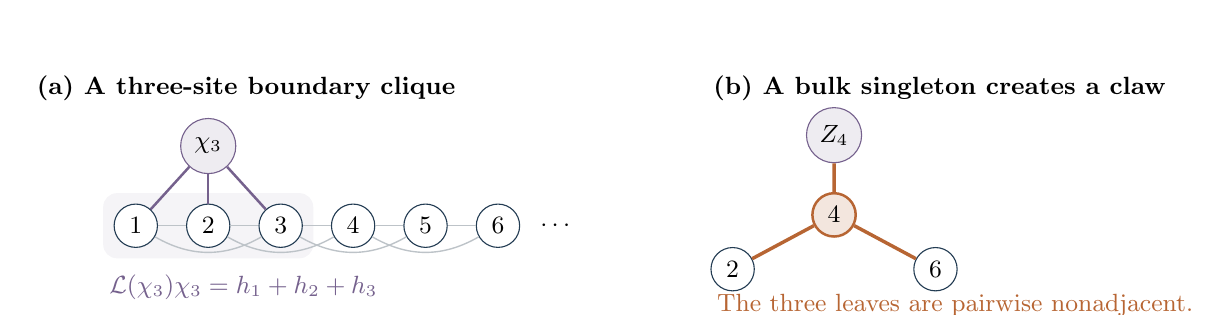
\begin{tikzpicture}[x=.92cm,y=.92cm]
\node[lab,font=\small\bfseries,anchor=west] at (-.5,1.9) {(a) A three-site boundary clique};
\fill[violet!7,rounded corners=5pt] (.55,-.45) rectangle (3.45,.45);
\foreach \i in {1,...,6}{\node[site] (c\i) at (\i,0) {$\i$};}
\foreach \i in {1,...,5}{\pgfmathtruncatemacro{\j}{\i+1}\draw[bg] (c\i)--(c\j);}
\foreach \i in {1,...,4}{\pgfmathtruncatemacro{\j}{\i+2}\draw[bg] (c\i) to[bend right=30] (c\j);}
\node[source] (sc) at (2,1.1) {$\chi_3$};
\foreach \i in {1,2,3}{\draw[se] (sc)--(c\i);}
\node[lab,anchor=west] at (6.45,0) {$\cdots$};
\node[lab,anchor=west,text=violet] at (.5,-.85) {$\LL(\chi_3)\chi_3=h_1+h_2+h_3$};
\begin{scope}[xshift=8.5cm]
\node[lab,font=\small\bfseries,anchor=west] at (-.4,1.9) {(b) A bulk singleton creates a claw};
\node[tsite] (bc) at (1.4,.15) {$4$};
\node[site] (bl) at (0,-.6) {$2$};
\node[site] (br) at (2.8,-.6) {$6$};
\node[source] (bs) at (1.4,1.25) {$Z_4$};
\draw[te] (bc)--(bl) (bc)--(br) (bc)--(bs);
\node[lab,anchor=west,text=target] at (-.35,-1.1) {The three leaves are pairwise nonadjacent.};
\end{scope}
\end{tikzpicture}
\caption{Why three boundary generators are accessible by this construction. The prefix cliques $K_1,K_2,K_3$ give valid sources, and differences of their density sums isolate $h_1,h_2,h_3$. By contrast, a source attached only to an interior vertex such as $4$ creates the displayed induced claw for $M\ge6$; the boundary-source theorem cannot be invoked there. The right-hand drawing shows only the induced four-vertex subgraph.}
\label{fig:clique}
\end{figure}

Replace $\chi_1$ and its paths by $\chi_k$ and paths rooted at $\alpha_k$ in \eqref{eq:Xi}. Denote the result $\Xi_k(u)$. The empty-path residual becomes
$Q_k(x)=\PP{k+1,M}(x)$; a nonempty path ending at $r$ still has residual $[r+3,M]$. Nothing changes in the spectrum or residue denominator:
\begin{equation}
 F_s^{(k)}=-\frac{\Xi_k(u_s)}{2u_s^2P'_s},\quad
 \chi_k(t)=Z_k^{\rm st}+\sum_se^{2\ii t\eps_s}F_s^{(k)},\quad
 S_k(t)=\left(\sum_s\eps_se^{2\ii t\eps_s}F_s^{(k)}\right)\chi_k(t).
 \label{eq:cliqueevol}
\end{equation}
Different $k$ generally give different mode operators, even though their energies agree. We compute each clique correlator in its own source basis and only then take differences.

Let $R_m^{(k)}$ be the source-to-$m$ path sum, again excluding the source and the final vertex from the weight. Set $R_m^{(k)}=1$ for $1\le m\le k$ and $R_m^{(k)}=0$ for $m\le0$. For $m>k$, resolve the two final gaps:
\begin{equation}
 \begin{aligned}
 \rho_{2,m}^{(k)}(y)&=-yB_{m-2}R_{m-2}^{(k)}(y),\\
 \rho_{1,m}^{(k)}(y)&=
 \begin{cases}
 -yB_k,&m=k+1,\\
 y^2B_{m-3}B_{m-1}R_{m-3}^{(k)}(y),&m\ge k+2,
 \end{cases}\\
 R_m^{(k)}(y)&=\rho_{1,m}^{(k)}(y)+\rho_{2,m}^{(k)}(y).
 \end{aligned}
 \label{eq:rhorec}
\end{equation}
Here an out-of-range factor $B_i$ with $i\le0$ means zero. The special first line of the piecewise definition is the direct path $\alpha_k\to k\to k+1$. It must not be replaced by a fictitious preceding physical step. Farther into the chain, \eqref{eq:rhorec} is exactly the scalar recurrence \eqref{eq:Rrec}. In particular
\begin{equation}
 R_3^{(2)}=-y(B_1+B_2),\qquad
 R_4^{(3)}=-y(B_2+B_3).
\end{equation}
The endpoint result immediately generalizes by replacing $R_M$ with $R_M^{(k)}$ in \eqref{eq:endcorr}, provided $M>k$.

\paragraph{Which source has a stationary part?}
It is the \emph{source}, not just the chain length, that decides this. The resolvent identity implies~\cite{FPV}
\begin{equation}
 (Z_k^{\rm st})^2=\lim_{x\to\infty}\frac{Q_k(x)}{P(x)}\,\one.
 \label{eq:stationary}
\end{equation}
Thus $Z_1^{\rm st}\ne0$ for $M\equiv0,2\pmod3$; $Z_2^{\rm st}\ne0$ only for $M\equiv0\pmod3$; and $Z_3^{\rm st}=0$. The stationary content therefore depends on which boundary source is chosen. The uniform weight \eqref{eq:weight} avoids that issue altogether.

\section{Moving the target into the bulk}
Let $j>k$. The same trace selection rule now reads
$V(p)\triangle V(q)=\{j\}$. The target must again be the final vertex of one path. It cannot be removed from the interior: the vertices on either side would have to become adjacent, contradicting inducedness of the longer path. Nor can the first physical vertex be removed, since the next vertex lies outside the source clique. Hence the pair is still $(\rho,\rho j)$.

What changes is only the residual graph. Define
\begin{equation}
 L_j(x)=\PP{j+3,M}(x),\qquad
 C_{2,j}(x)=\PP{j+1,M}(x),\qquad
 C_{1,j}(x)=\PP{j+2,M}(x).
 \label{eq:tails}
\end{equation}
The longer path always leaves $L_j$. If the shorter path ends at $j-2$, its residual is $C_{2,j}$; if it ends at $j-1$, its residual is $C_{1,j}$. These are the only possibilities, depicted in Fig.~\ref{fig:tails}.

\begin{figure}[t]
\centering
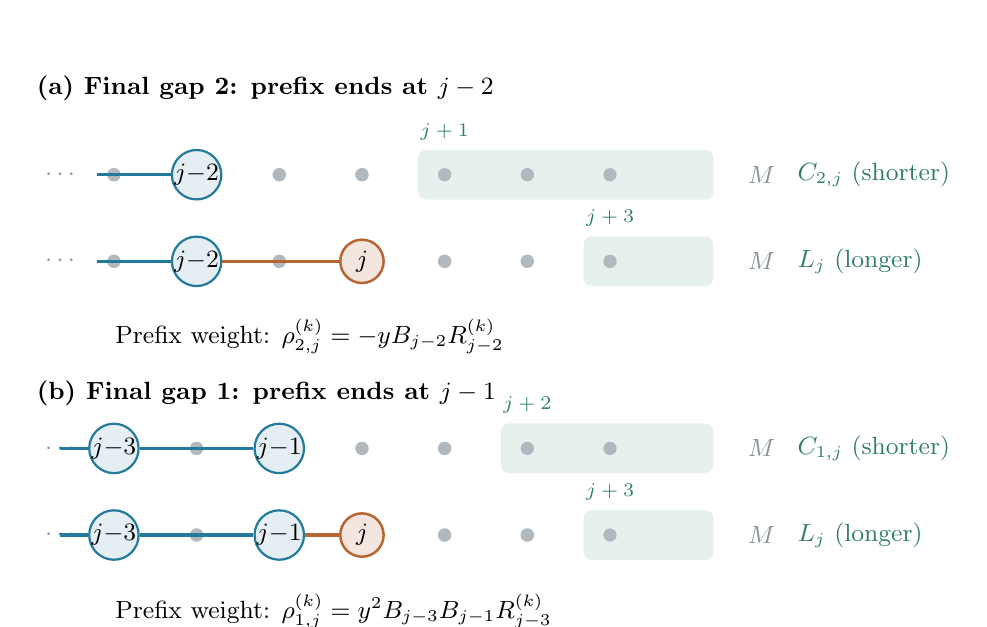
\begin{tikzpicture}[x=1.05cm,y=.88cm]
\node[lab,font=\small\bfseries,anchor=west] at (-1.05,2.6) {(a) Final gap 2: prefix ends at $j-2$};
\node[lab,font=\small\bfseries,anchor=west] at (-1.05,-1.8) {(b) Final gap 1: prefix ends at $j-1$};
% Common local axis: j-3, j-2, j-1, j, j+1, j+2, j+3, ...
\foreach \yy/\nn in {1.35/a,.1/b,-2.6/c,-3.85/d}{
 \foreach \i in {0,...,6}{\node[circle,fill=grey!40,inner sep=1.7pt] (\nn\i) at (\i,\yy) {};}
 \node[lab,anchor=east,text=grey] at (-.3,\yy) {$\cdots$};
 \node[lab,anchor=west,text=grey] at (7.55,\yy) {$M$};
}
% Residuals
\fill[tailgreen!12,rounded corners=3pt] (3.68,.99) rectangle (7.25,1.71);
\fill[tailgreen!12,rounded corners=3pt] (5.68,-.26) rectangle (7.25,.46);
\fill[tailgreen!12,rounded corners=3pt] (4.68,-2.96) rectangle (7.25,-2.24);
\fill[tailgreen!12,rounded corners=3pt] (5.68,-4.21) rectangle (7.25,-3.49);
\foreach \yy/\nn in {1.35/a,.1/b,-2.6/c,-3.85/d}{
 \foreach \i in {0,...,6}{\node[circle,fill=grey!65,inner sep=1.7pt] (\nn\i) at (\i,\yy) {};}
}
\node[psite] (a1) at (1,1.35) {$j{-}2$};
\draw[pe] (-.2,1.35)--(a1);
\node[psite] (b1) at (1,.1) {$j{-}2$};
\node[tsite] (b3) at (3,.1) {$j$};
\draw[pe] (-.2,.1)--(b1);\draw[te] (b1)--(b3);
\node[psite] (c0) at (0,-2.6) {$j{-}3$};
\node[psite] (c2) at (2,-2.6) {$j{-}1$};
\draw[pe] (-.65,-2.6)--(c0)--(c2);
\node[psite] (d0) at (0,-3.85) {$j{-}3$};
\node[psite] (d2) at (2,-3.85) {$j{-}1$};
\node[tsite] (d3) at (3,-3.85) {$j$};
\draw[pe] (-.65,-3.85)--(d0)--(d2);\draw[te] (d2)--(d3);
\node[font=\scriptsize,text=tailgreen,above] at (4,1.71) {$j+1$};
\node[font=\scriptsize,text=tailgreen,above] at (6,.46) {$j+3$};
\node[font=\scriptsize,text=tailgreen,above] at (5,-2.24) {$j+2$};
\node[font=\scriptsize,text=tailgreen,above] at (6,-3.49) {$j+3$};
\node[lab,text=tailgreen,anchor=west] at (8.15,1.35) {$C_{2,j}$ (shorter)};
\node[lab,text=tailgreen,anchor=west] at (8.15,.1) {$L_j$ (longer)};
\node[lab,text=tailgreen,anchor=west] at (8.15,-2.6) {$C_{1,j}$ (shorter)};
\node[lab,text=tailgreen,anchor=west] at (8.15,-3.85) {$L_j$ (longer)};
\node[lab,anchor=west] at (-.1,-.98) {Prefix weight: $\rho_{2,j}^{(k)}=-yB_{j-2}R_{j-2}^{(k)}$};
\node[lab,anchor=west] at (-.1,-4.95) {Prefix weight: $\rho_{1,j}^{(k)}=y^2B_{j-3}B_{j-1}R_{j-3}^{(k)}$};
\end{tikzpicture}
\caption{The entire bulk modification is local at the target. Shaded intervals are the residual graphs, not part of the selected path. Adding $j$ shifts the start of the residual interval to $j+3$. The second prefix-weight formula is the generic one; at $j=k+1$ the prefix is just the clique vertex $k$, and its weight is $-yB_k$ as in \eqref{eq:rhorec}. The labels $j\pm a$ denote positions along the chain; grey dots are unselected vertices.}
\label{fig:tails}
\end{figure}

Write
\begin{equation}
 \Delta_{a,j}(u,v)
 =uL_j(u^2)C_{a,j}(v^2)-vC_{a,j}(u^2)L_j(v^2),\qquad a=1,2.
 \label{eq:Delta}
\end{equation}
The path-pair overlap is then
\begin{equation}
 \boxed{\Kern_{kj}(u,v):=\av{\Xi_k(u)\Xi_k(v)h_j}
 =B_j\!\left[\rho_{2,j}^{(k)}(uv)\Delta_{2,j}(u,v)
 +\rho_{1,j}^{(k)}(uv)\Delta_{1,j}(u,v)\right],\quad j>k.}
 \label{eq:bulkkernel}
\end{equation}
To derive it, repeat the endpoint sign calculation for each prefix $\rho$. In one ordering the extra factor $-u$ belongs to the longer path, whose residual is $L_j(u^2)$; the shorter path carries $C_{a,j}(v^2)$. The reversed ordering gives the other term with the opposite sign. Summing the common prefix weights gives $\rho_{a,j}^{(k)}$. This proves \eqref{eq:bulkkernel} for arbitrary spectral parameters. It also explains why a single polynomial in $uv$ no longer suffices: the two residual tails are evaluated separately at $u^2$ and $v^2$.

\begin{theorem}[Boundary-clique--bulk correlator]
For $1\le k\le\min(3,M)$ and $j>k$, let $\W$ be \eqref{eq:weight}, let the path weights be generated by \eqref{eq:rhorec}, and let the tails be \eqref{eq:tails}. Then
\begin{equation}
 \boxed{D_{kj}(t):=\av{S_k(t)h_j}
 =\sum_{s,r\in\Sig}\W_{sr}(t)\Kern_{kj}(u_s,u_r).}
 \label{eq:main}
\end{equation}
\end{theorem}
\begin{proof}
Equation~\eqref{eq:cliqueevol} reduces the calculation to two source components. Since $j\notin K_k$, no single source path has physical vertex set $\{j\}$, and therefore $\av{F_s^{(k)}\chi_kh_j}=0$. Eliminate $Z_k^{\rm st}$ exactly as in \eqref{eq:zeroelim}. Finally,
\[
 \av{F_s^{(k)}F_r^{(k)}h_j}
 =\frac{\Kern_{kj}(u_s,u_r)}{4u_s^2u_r^2P'_sP'_r}.
\]
Multiplication by $\eps_s$ and the time phases gives \eqref{eq:main}.
\end{proof}

\paragraph{Two useful checks.}
At $j=M$ all three tails are $1$, so
$\Kern_{kM}=B_M(u-v)R_M^{(k)}(uv)$, recovering the endpoint calculation. At the other extreme, $k=3,j=4$ gives
$\rho_{2,4}^{(3)}=-yB_2$ and $\rho_{1,4}^{(3)}=-yB_3$.
Thus the formula includes the first site beyond the boundary block; no artificial condition $j\ge k+3$ is required. The exceptional initial weight in \eqref{eq:rhorec} is essential for this extension.

\section{Individual generators, reflection, and nearby targets}
With $D_{0j}=0$, taking differences of the nested source sums gives the desired densities:
\begin{equation}
 \boxed{\av{h_m(t)h_j}=D_{mj}(t)-D_{m-1,j}(t),
 \qquad m=1,2,3,\quad j\ge4.}
 \label{eq:individual}
\end{equation}
Both terms use the same roots of $P$, but their path weights are those of their own source cliques. This is the partial inverse problem in its most useful form: the dynamics of the boundary observable is simple, and only the appropriate two-source-component overlap of the bulk observable is needed. We never assert that $h_j$ itself is quadratic in a fixed set of hidden modes.

For reflected couplings $\bar b_i=b_{M+1-i}$, write $\bar D$ for the same formulas evaluated on the reflected chain. Trace cyclicity gives
\begin{equation}
 \av{h_j(t)h_{M-r+1}}
 =\bar D_{r,M+1-j}(-t)-\bar D_{r-1,M+1-j}(-t),\qquad r=1,2,3.
 \label{eq:reflection}
\end{equation}
Thus the last three terms are equally accessible. In this real representation the correlators are even in time, so the minus sign may also be dropped after evaluation.

\paragraph{Targets inside the source clique.}
For completeness, the phrase ``every term'' includes $j\le k$. In this case the only surviving pair is the empty path and the one-vertex path $(j)$. Consequently the kernel is instead
\begin{equation}
 \Kern_{kj}(u,v)=B_j\left[uL_j(u^2)Q_k(v^2)-vQ_k(u^2)L_j(v^2)\right],\qquad j\le k.
 \label{eq:insidekernel}
\end{equation}
Now $\av{\Xi_k(u)\chi_kh_j}=uB_jL_j(u^2)$ is nonzero. Keeping this elementary term when eliminating the stationary part gives
\begin{equation}
 D_{kj}(t)=\sum_{s,r}\W_{sr}(t)\Kern_{kj}(u_s,u_r)
 -\frac{B_j}{2}\sum_s\frac{L_j(u_s^2)}{u_s^2P'_s}e^{2\ii t/u_s},\qquad j\le k.
 \label{eq:insidecorr}
\end{equation}
Equations~\eqref{eq:main} and \eqref{eq:insidecorr}, followed by the same finite difference, therefore cover every target $1\le j\le M$, including autocorrelations. At $t=0$ they give $D_{kj}(0)=B_j\mathbf1_{j\le k}$.

\paragraph{Opposite boundary blocks need no new machinery.}
For $T_\ell=\{M-\ell+1,\ldots,M\}$ and $M\ge6$, summing \eqref{eq:bulkkernel} over the target block gives
\begin{align}
 \av{\Xi_k(u)\Xi_k(v)\sum_{j\in T_\ell}h_j}
 &=(u-v)\mathcal R_{k\ell}(uv),\notag\\
 \mathcal R_{k1}(y)&=B_MR_M^{(k)}(y),\notag\\
 \mathcal R_{k2}(y)&=B_{M-1}R_{M-1}^{(k)}(y)-yB_MB_{M-2}R_{M-2}^{(k)}(y),\notag\\
 \mathcal R_{k3}(y)&=B_{M-2}R_{M-2}^{(k)}(y)-yB_{M-1}B_{M-3}R_{M-3}^{(k)}(y).
 \label{eq:firsthit}
\end{align}
These are first-hit path sums: the first vertex encountered in the target clique carries $B_j$, while each preceding vertex carries $-yB_i$. An induced path can first enter $T_2$ at $M-1$, or jump from $M-2$ to $M$; it can first enter $T_3$ at $M-2$, or jump from $M-3$ to $M-1$. These are exactly the displayed terms. In the overlap sum, contributions that continue inside the clique cancel the residual-tail terms. Equivalently, substitution of the degree-zero and degree-one endpoint tails into \eqref{eq:bulkkernel}, followed by \eqref{eq:rhorec}, verifies all three identities directly. The correlator is $\sum_{s,r}\W_{sr}(t)(u_s-u_r)\mathcal R_{k\ell}(u_su_r)$; differences in both block sizes isolate any of the nine opposite-edge pairs.

\section{Computation, checks, and the extent of the result}
\paragraph{Polynomial work, without enumerating paths.}
The path expansion is a proof device, not the computational algorithm. Build $P$ by \eqref{eq:Prec} and determine its $S=O(M)$ roots. At each root, generate all right tails by the backward recurrence
\begin{equation}
 \PP{a,M}(x)=\PP{a+1,M}(x)-xB_a\PP{a+3,M}(x).
\end{equation}
For each signed pair $(s,r)$, run the scalar recurrence \eqref{eq:rhorec} at $y=u_su_r$, evaluate the desired kernel, and sum \eqref{eq:main}. For a fixed edge--target pair this takes $O(MS^2)=O(M^3)$ arithmetic operations after the spectral data are obtained; storing its $O(S^2)$ coefficients reduces each additional time evaluation to $O(S^2)$. All targets can share the same path sweeps. A conventional polynomial-coefficient/root-finding implementation also has polynomial arithmetic cost. These are arithmetic bounds, not uniform bit-complexity or floating-point stability guarantees: large chains, strongly separated couplings, or clustered roots may require higher precision.

\paragraph{Independent verification.}
The path recurrence, resolvent identity, all-target overlap, and opposite-clique sums were checked by enumerating induced paths and multiplying graph-Clifford words in exact integer arithmetic, through $M=18$ (102, 51, 509, and 117 checks, respectively). The finite-time formulas were separately compared with direct commutator evolution on the ordered-word basis for $2\le M\le12$, all allowed $k,j$, uniform, nonuniform and random signed couplings, and four times. Across 2,748 scalar comparisons the maximum absolute discrepancy was $1.05\times10^{-13}$. Reproducible scripts and parameter choices accompany the source files. These checks support, but do not replace, the analytic derivation. Useful implementation tests are
\begin{equation}
 \av{h_i h_j}=B_i\delta_{ij},\qquad
 \sum_{j=1}^{M}\av{h_i(t)h_j}=B_i,
\end{equation}
the second following from conservation of $\HH$.

\paragraph{Relation to existing methods.}
The spectral polynomial and hidden fermions originate in Refs.~\cite{Fendley,Elman,Chapman}; boundary inverse formulas and selected real-time correlators were obtained in Ref.~\cite{VMP}. The essential input here is the explicit path-product resolvent of Ref.~\cite{FPV}, whose general proof is not repeated. The additional reduction is at the level of the \emph{density overlap}: trace orthogonality leaves two terminal path configurations, and hence the scalar formulas \eqref{eq:bulkkernel}--\eqref{eq:main}.

Polynomial contraction is also consistent with the matrix-product-operator approach to mode expectation values developed for FFD circuits in Ref.~\cite{Circuits}. In the Hamiltonian setting, the finite-range independent-set transfer recurrence has a finite-memory tensor-network representation, so a fixed product of mode operators with a local insertion can likewise be contracted with polynomial work. This gives an alternative complexity argument; the path calculation provides the explicit scalar kernel rather than a claim of first establishing polynomial simulability for boundary observables. Recent work on bulk generalized-Gibbs-ensemble expectations and quench dynamics~\cite{Quench} addresses a different question from the finite-time, infinite-temperature cross-correlators considered here. The distinction between the physical-mode algebra and degeneracy degrees of freedom is developed in Ref.~\cite{VP}.

\paragraph{What is not solved.}
The three-site reach comes from the nested boundary cliques, not from a claim that all densities have a quadratic expression in one common fermion basis. The block $\{1,2,3,4\}$ is not a clique, so the same argument does not produce $S_4$. Attaching a source only to a bulk site generally creates a claw, as Fig.~\ref{fig:clique}(b) shows. Thus, when both densities lie outside the accessible edge blocks, a correlator such as $\av{h_4(t)h_{M-3}}$ for $M\ge10$ is not determined by these formulas. This is a limitation of the construction, not an impossibility theorem for bulk--bulk dynamics. In particular, no truncation of a generic bulk operator to quadratic or quartic physical-fermion sectors has been assumed.

The central lesson is that a correlation function can be simpler than the inverse problem for either of its factors in a fixed fermionic dictionary. A boundary source supplies the dynamics; the normalized trace selects a small part of the target operator; and induced-path geometry evaluates that part with scalar recurrences. This is precisely the partial inverse problem solved here.

\begin{thebibliography}{9}\small
\bibitem{Fendley}
P.~Fendley, \emph{Free fermions in disguise}, J. Phys. A: Math. Theor. \textbf{52}, 335002 (2019), \href{https://doi.org/10.1088/1751-8121/ab305d}{doi:10.1088/1751-8121/ab305d}; arXiv:1901.08078.
\bibitem{Elman}
S.~J.~Elman, A.~Chapman and S.~T.~Flammia, \emph{Free fermions behind the disguise}, Commun. Math. Phys. \textbf{388}, 969--1003 (2021), \href{https://doi.org/10.1007/s00220-021-04220-w}{doi:10.1007/s00220-021-04220-w}; arXiv:2012.07857.
\bibitem{Chapman}
A.~Chapman, S.~J.~Elman and R.~L.~Mann, \emph{A unified graph-theoretic framework for free-fermion solvability}, \href{https://arxiv.org/abs/2305.15625}{arXiv:2305.15625} (2023).
\bibitem{VMP}
I.~Vona, M.~Mesty\'an and B.~Pozsgay, \emph{Exact real-time dynamics with free fermions in disguise}, Phys. Rev. B \textbf{111}, 144306 (2025), \href{https://doi.org/10.1103/PhysRevB.111.144306}{doi:10.1103/PhysRevB.111.144306}; arXiv:2405.20832.
\bibitem{FPV}
K.~Fukai, B.~Pozsgay and I.~Vona, \emph{Solving models with generalized free fermions II: Path-product expansion and conserved charges}, \href{https://arxiv.org/abs/2605.31453v2}{arXiv:2605.31453v2} (2026), especially Secs.~3.2--3.4 and 8.1. The path-product theorem and source-residue decomposition are used as established inputs.
\bibitem{Circuits}
D.~Sz\'asz-Schagrin, D.~Cristani, L.~Piroli and E.~Vernier, \emph{Construction and simulability of quantum circuits with free fermions in disguise}, Quantum Sci. Technol. \textbf{11}, 015044 (2026), \href{https://doi.org/10.1088/2058-9565/ae390d}{doi:10.1088/2058-9565/ae390d}; arXiv:2509.22585.
\bibitem{Quench}
D.~Sz\'asz-Schagrin, P.~Bayona-Pena, L.~Piroli and E.~Vernier, \emph{Correlation and entanglement dynamics of free fermions in disguise}, \href{https://arxiv.org/abs/2607.02359v2}{arXiv:2607.02359v2} (2026).
\bibitem{VP}
E.~Vernier and L.~Piroli, \emph{The Hilbert-space structure of free fermions in disguise}, J. Stat. Mech. \textbf{2026}, 013101 (2026), \href{https://doi.org/10.1088/1742-5468/ae29f5}{doi:10.1088/1742-5468/ae29f5}; arXiv:2507.15959.
\end{thebibliography}
\end{document}
